%%%%%%%%%%%%%%%%%%%%%%%%%%%%%%%%%%%%%%%%%
% Journal Article
% LaTeX Template
% Version 1.3 (9/9/13)
%
% This template has been downloaded from:
% http://www.LaTeXTemplates.com
%
% Original author:
% Frits Wenneker (http://www.howtotex.com)
%
% License:
% CC BY-NC-SA 3.0 (http://creativecommons.org/licenses/by-nc-sa/3.0/)
%
%%%%%%%%%%%%%%%%%%%%%%%%%%%%%%%%%%%%%%%%%

%----------------------------------------------------------------------------------------
%	PACKAGES AND OTHER DOCUMENT CONFIGURATIONS
%----------------------------------------------------------------------------------------

\documentclass[twoside]{article}

\usepackage{lipsum} % Package to generate dummy text throughout this template
\usepackage[french]{babel}

\usepackage[utf8]{inputenc}

\usepackage[sc]{mathpazo} % Use the Palatino font
\usepackage[T1]{fontenc} % Use 8-bit encoding that has 256 glyphs
\linespread{1.05} % Line spacing - Palatino needs more space between lines
\usepackage{microtype} % Slightly tweak font spacing for aesthetics

\usepackage[hmarginratio=1:1,top=32mm,columnsep=20pt]{geometry} % Document margins
\usepackage{multicol} % Used for the two-column layout of the document
\usepackage[hang, small,labelfont=bf,up,textfont=it,up]{caption} % Custom captions under/above floats in tables or figures
\usepackage{booktabs} % Horizontal rules in tables
\usepackage{float} % Required for tables and figures in the multi-column environment - they need to be placed in specific locations with the [H] (e.g. \begin{table}[H])
\usepackage{hyperref} % For hyperlinks in the PDF

\usepackage{lettrine} % The lettrine is the first enlarged letter at the beginning of the text
\usepackage{paralist} % Used for the compactitem environment which makes bullet points with less space between them
\usepackage{graphicx}

\usepackage{abstract} % Allows abstract customization
\renewcommand{\abstractnamefont}{\normalfont\bfseries}
\renewcommand{\abstractname}{Résumé} % Set the "Abstract" text to bold
\renewcommand{\abstracttextfont}{\normalfont\small\itshape} % Set the abstract itself to small italic text

\usepackage{titlesec} % Allows customization of titles
\renewcommand\thesection{\Roman{section}} % Roman numerals for the sections
\renewcommand\thesubsection{\arabic{subsection}.\arabic{subsection}} % Roman numerals for subsections
\titleformat{\section}[block]{\bfseries\large\scshape\centering}{\thesection.}{1em}{} % Change the look of the section titles
\titleformat{\subsection}[block]{\bfseries\large}{\thesubsection.}{1em}{} % Change the look of the section titles

\usepackage{fancyhdr} % Headers and footers
\pagestyle{fancy} % All pages have headers and footers
\fancyhead{} % Blank out the default header
\fancyfoot{} % Blank out the default footer
\renewcommand{\headrulewidth}{0pt} %pour enlever la ligne du header
%\fancyhead[C]{titre, date, noms...	} % Custom header text
\fancyfoot[RO,LE]{\thepage} % Custom footer text


%agrandissement de la zone de texte
\addtolength{\oddsidemargin}{-1cm}
\addtolength{\evensidemargin}{-1cm}
\addtolength{\textwidth}{2cm}

%pour les maths
\usepackage{amsmath}
\usepackage{amsfonts}
\usepackage{todonotes}
%----------------------------------------------------------------------------------------
%	TITLE SECTION
%----------------------------------------------------------------------------------------

\title{\vspace{-15mm}\fontsize{24pt}{10pt}\selectfont\textbf{Identification de défauts par onde de Lamb}} % Article title

\author{
\large
{Alice \textsc{Dinsenmeyer} \& Thomas \textsc{Lechat}}\\[2mm] % Your name %\thanks{}
%\normalsize University of California \\ % Your institution
%\normalsize \href{mailto:john@smith.com}{john@smith.com} % Your email address
\vspace{-5mm}
}
\date{}

%----------------------------------------------------------------------------------------

\begin{document}

\maketitle % Insert title

\thispagestyle{fancy} % All pages have headers and footers

%----------------------------------------------------------------------------------------
%	ABSTRACT
%----------------------------------------------------------------------------------------

\begin{abstract}


\end{abstract}

%----------------------------------------------------------------------------------------
%	ARTICLE CONTENTS
%----------------------------------------------------------------------------------------

\begin{multicols}{2} % Two-column layout throughout the main article text

\section{Introduction}
Différents types d'ondes élastiques sont connus dans la propagation dans la matière. Ces ondes peuvent être séparées en 2 catégories: les ondes de locales (longitudinales et transversales) qui sont solutions de l'équation d'onde en milieu infini et les ondes dites modales (à ne pas confondre avec la théorie modale) qui apparaissent quand on prend en compte les conditions limites au interfaces. Les ondes de cette seconde catégorie sont constituées d'ondes longitudinales (L) et transversales (T) qui se recombinent quand on prend en compte les conditions limites.  Dans cette  catégorie, on peut citer les ondes de Rayleigh pour un matériau semi-infini avec une interface vers le vide ou encore les ondes de Lamb pour une plaque dans le vide (2 interfaces vide-solide). Ces dernières ont été mise en évidence par Lamb en 1917 \cite{Lamb}, se sont des ondes guidées se propageant dans la plaque.
C'est sur l'utilisation des ondes de Lamb dans le contrôle non destructif que porte se document.

%------------------------------------------------
\section{Les ondes de Lamb}
Afin de mettre en évidence l’existence d'une guidée dans une plaque, on considère une plaque d'épaisseur $h$, \emph{in vacuo}, dans laquelle se propage des ondes T et L. L'ensemble des ondes T peuvent être écrites sous la forme de 2 onde équivalente (une se propageant vers le haut, l'autre vers le bas), de même pour les ondes L. Cela est possible car selon la loi de Snell-Descartes, la direction des vecteurs d'ondes restent inchangés pendant la propagation. Un schéma explicatif est représenté figure ~\ref{fig1}.


\begin{figure}[H]
\centering
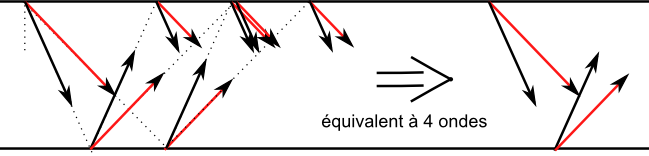
\includegraphics[scale=0.5]{./images/lamb_expli.png}
\caption{\label{fig1} Schéma de la propagation des ondes dans une plaque in vacuo.}
\end{figure}

Il y a donc 4 inconnus au problèmes (correspondant au 4 amplitudes des ondes). Après applications des conditions limites (contraintes normales et tangentielles nulles au interfaces car la plaque est \emph{in vacuo}, on obtient un système de 4 équations à 4 inconnus. Il est ensuite facile d'en tirer l'équation de dispersion des ondes dans le milieu en prenant le determinant de la matrice du système d'équation. Celle-ci montre qu'il existe 2 types de modes après recombinaison des ondes T et L: les modes symétriques (notés $S_i$) et anti-symétriques (notés $A_i$) qui correspondent à des ondes de compression et des ondes de flexion. Les champs de déplacements de ses 2 types de modes sont représentés sur le schéma \ref{fig2}.

\begin{figure}[H]
\centering
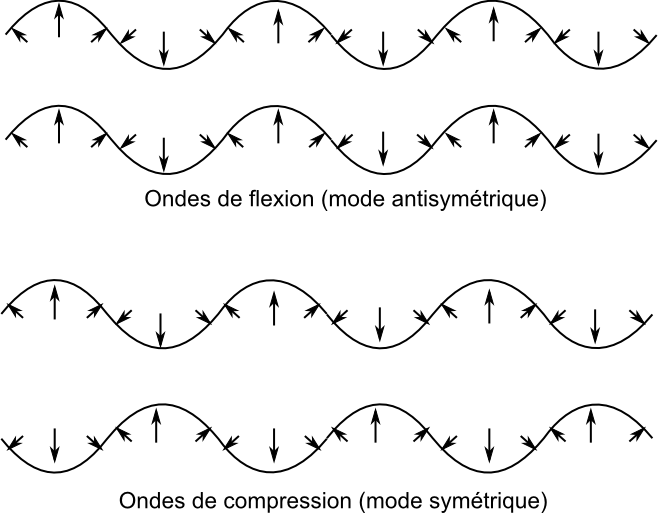
\includegraphics[scale=0.4]{./images/modes.png}
\caption{\label{fig2} Déplacements des 2 modes des ondes de Lamb.}
\end{figure}


\subsection{Courbes de dispersion}

Les courbes de dispersions des ondes de Lamb peuvent être représentés de différentes manières. Dans la figure ~\ref{fig3}, les vitesses de phases sont présentées en fonction de $f.h$ ou $h$ est l'épaisseur de la plaque. 

%\begin{figure}
%\centering
%\includegraphics[scale=0.6]{./images/courbes_dispersion.png}
%\caption{\label{fig3} Courbes de dispersion des ondes de Lamb pour une plaque en aluminium de 5.6mm d'épaisseur.}
%\end{figure}
\todo{ajouter la courbe}



%------------------------------------------------

\section{Mesure de temps de vol sur une plaque d'acier}
Dans cette section, une onde de Lamb est générée au moyen d'un capteur piézo-électrique dans une plaque d'aluminium de $d = 5.6mm$ d'épaisseur. Le transducteur est placé en incidence normale sur la plaque (avec un couplant), c'est donc les ondes générées par le bord du transducteur qui rayonnent dans la plaque et se combinent pour former les ondes de Lamb.
\bigskip
Stricto senso, se sont des ondes de Lamb généralisées qui sont produites: c'est la généralisation des ondes de Lamb pour une plaque dans un fluide léger. Un rayonnement de ces ondes est possible dans le fluide. 
Le but étant de valider les courbes trouvées précédemment, le temps de vol d'impulsions pour différentes fréquences (bursts de 3 cycles) sont relevés avec un deuxième capteur piézo-électriques placé à une distance connue de l'émetteur. Les points représentés figure ~\ref{fig3} sont obtenues à partir des vitesses calculées en fonction des temps de vols.
%
%\begin{figure}
%\centering
%\includegraphics[scale=0.5]{./images/courbe_plus_mesure.png}
%\caption{\label{fig3} Mesure de la vitesse de phase pour une plaque d'aluminium de $d=5.56mm$ d'épaisseur.}
%\end{figure}
\todo{faire la note}

\subsection{Ondes de fuites}
couplant+ capteur = onde de fuite


%------------------------------------------------

\section{Utilisation d'un EMAT pour contrôler un tuyau}




\section{Conclusion}
%----------------------------------------------------------------------------------------
%	REFERENCE LIST
%----------------------------------------------------------------------------------------

\begin{thebibliography}{99} % Bibliography - this is intentionally simple in this template

\bibitem[Lamb]{Lamb}
Lamb, H. 1917.
\newblock"On Waves in an Elastic Plate.
\newblock {\em Proc. Roy. Soc. London, Ser. A 93, 114–128}
 
\end{thebibliography}

%----------------------------------------------------------------------------------------

\end{multicols}

\end{document}
